\documentclass[12pt,a4paper,oneside]{article} %стиль оформления - статья с параметрами: шрифт 12, формат бумаги А4, печать с одинаковыпи полями на всех страницах - oneside
\usepackage[T2A]{fontenc} %поддержка кириллицы
\usepackage[utf8]{inputenc} %кодировка символов
\usepackage[english,russian]{babel} %пакет поддержки русского языка с элементами английского
\frenchspacing
\usepackage[dvips]{graphicx} %разрешить включение PostScript-графики
\graphicspath{{images/}}
\usepackage{setspace} %"умное" расстояние между строк
\usepackage[usenames,dvipsnames]{color}
\usepackage{hhline} %работа с таблицами
\usepackage[12pt]{extsizes} %размер шрифта
\usepackage{fancyhdr} %установка колонтитулов

\usepackage{geometry} %ручная установка полей
\geometry{top=1cm} %поле сверху
\geometry{bottom=1cm} %поле снизу
\geometry{left=2cm} %поле слева
\geometry{right=2cm} %поле справа

\begin{document}
\singlespacing % межстрочный одиночный интервал для всего текста
\pagestyle{empty} % нумерация выкл.

%Н:задание на уир и кп
\newpage
\begin{center}
МИНИСТЕРСТВО ОБРАЗОВАНИЯ И НАУКИ РОССИЙСКОЙ ФЕДЕРАЦИИ

Федеральное государственное бюджетное образовательное учреждение \linebreak
высшего профессионального образования

\textbf{"Национальный исследовательский ядерный университет "МИФИ"}
\\[10pt]

\begin{figure}[h]

\includegraphics[trim=-10 40 30 0,width=0.25\linewidth]{mifi}
\end{figure}

ФАКУЛЬТЕТ КИБЕРНЕТИКИ
\\[15pt]

КАФЕДРА ИНФОРМАЦИОННЫЕ ТЕХНОЛОГИИ
\\[60pt]

\LARGE{\textbf{ПОЯСНИТЕЛЬНАЯ ЗАПИСКА}}
\\[10pt]

\large{к курсовому проекту на тему:}
\\[10pt]

\large{\underline{Разработка модуля преобразования геоданных из формата\hspace{4cm}} \linebreak
\underline{OpenStreetMap в формат OpenGIS\hspace{9,36cm}}}
\\[50pt]
\end{center}

\begin{flushleft}
\large{Группа \underline{К7-361\hspace{13,75cm}}

Студент \underline{\hspace{9,1cm} (\hspace{0,5cm} Лаврентьева М.О. \hspace{0,5cm})}}

\hspace{6,5cm}\small{(подпись)}\hspace{5,2cm}\small{(Ф.И.О.)}

\large{Руководитель \underline{\hspace{7,92cm} (\hspace{0,84cm} Муравьёв С.К. \hspace{0,84cm})}}

\hspace{6,5cm}\small{(подпись)}\hspace{5,2cm}\small{(Ф.И.О.)}

\large{Оценка \underline{\hspace{15,2cm}}

Члены комиссии \underline{\hspace{7,3cm} ({\hspace{5,3cm}})}}

\hspace{6,5cm}\small{(подпись)}\hspace{5,2cm}\small{(Ф.И.О.)}

\large{\hspace{3,7cm} \underline{\hspace{7,3cm} ({\hspace{5,3cm}})}}

\hspace{6,5cm}\small{(подпись)}\hspace{5,2cm}\small{(Ф.И.О.)}

\large{\hspace{3,7cm} \underline{\hspace{7,3cm} ({\hspace{5,3cm}})}}

\hspace{6,5cm}\small{(подпись)}\hspace{5,2cm}\small{(Ф.И.О.)}

\large{\hspace{3,7cm} \underline{\hspace{7,3cm} ({\hspace{5,3cm}})}}

\hspace{6,5cm}\small{(подпись)}\hspace{5,2cm}\small{(Ф.И.О.)}

\end{flushleft}
\begin{center}
\vfill
\large{\textbf{Москва 2011}}
\end{center}
%K: титульный лист
%Н: литература
\newpage
\subsubsection*{Литература}
\begin{itemize}
\item Львовский С.М. Набор и верстка в пакете LaTeX - 3-е изд. \linebreak
Электронное издание, 2003.
\item Сандра Э.Эдди XML Справочник, изд. 'ПИТЕР', 1999, 480с.
\item Конспект лекций по теории программирования C++.
\item Бланшет Ж., Саммерфилд М. Qt4 программирование GUI на C++ - 2-е изд.\linebreak
Изд. 'КУДИЦ-ПРЕСС', Москва, 2008, 736 с.
\item Документация PostgreSQL. http://postgresql.ru.net/docs.html
\item Документация XML
\end{itemize}
%К: литература
%Н: оглавление
\newpage
\tableofcontents

%К: оглавление
%Н: введение
\newpage
\section{Введение}

\large{

В настоящее время широкое распространение в информационных \linebreak %борьба с переносами
технологиях получили геоинформационные системы (ГИС). ГИС  \linebreak %борьба с переносами
представляет собой аппаратно-программный человеко-машинный \linebreak %борьба с переносами
комплекс, обеспечивающий сбор, обработку, отображение и \linebreak
распространение геоданных.

Понятие геоданные (пространственные данные, географические \linebreak
данные) включает в себя цифровые данные о пространственных \linebreak
объектах, сведения об их местоположении и свойствах, пространственных \linebreak
и непространственных атрибутах.

ГИС позволяет эффективно и комплексно  использовать \linebreak
совершенно различные геоданные при решении научных и прикладных \linebreak
географических задач, связанных с инвентаризацией, анализом, \linebreak
моделированием, прогнозированием и управлением окружающей средой и \linebreak
территориальной организацией общества.

Термин ГИС используется и в более узком смысле — как инструмент \linebreak
(программный продукт), позволяющий пользователям искать, анализировать \linebreak
и редактировать цифровые карты, а также получать различную \linebreak
дополнительную информацию. Наиболее известные и часто используемые\linebreak
современные ГИС - это ArcGIS, MapInfo, а также Google Maps, Yandex-карты.

Данная учебно-исследовательская работа посвящена рассмотрению задачи \linebreak
сбора, обмена и хранения геоданных.

Исходные картографические данные для учебно-исследовательской\linebreak
работы будут получены из открытого источника в интернете \linebreak
OpenStreetMap.org в формате OSM XML.

Однако обмен и хранение пространственных данных требует развитой \linebreak
и всеобъемлющей системы стандартов представления геоданных. \linebreak
Такой системой стандартов для многих приложений на данный момент \linebreak
является формат Open Geospatial Consortium (OGC) (или сокращенно \linebreak
OpenGIS). Таким образом, для дальнейшего анализа и представления \linebreak
полученных геоданных их необходимо представить в данном формате \linebreak
(в формате OpenGIS).

\underline{Целью работы} является описание алгоритма и реализация \linebreak
функционала модуля преобразования геоданных из формата \linebreak
OpenStreetMap в формат OpenGIS.}

\underline{Задачи работы}:
\begin{enumerate}
\item Изучить структуру XML-документа с геоданными в формате OSM.

  В данном пункте предполагается изучить структуру и синтаксис \linebreak
  XML-документа. Выявить и описать особенности структуры и \linebreak
  синтаксиса документа OSM XML. А также описать какие \linebreak
  сведения о местоположении и свойствах пространственных данных \linebreak
  можно получить из документа OSM XML.
\item Построить XPath-запросы для извлечения геоданных об объектах \linebreak
заданного типа.

  В данном пункте предполагается изучить синтаксис языка запросов \linebreak
  XPath, овладеть навыками построения типовых XPath-запросов и \linebreak
  построить XPath-запросы к документу OSM XML для извлечения \linebreak
  необходимых сведений о пространственных данных.
\item Изучить стандарт OpenGIS и разработать структуру базы \linebreak
данных для хранения геоданных в формате OpenGIS.

  Здесь планируется изучить особенности СУБД PostgreSQL и её \linebreak
  расширения PostGIS для работы с геоданными в формате OpenGIS, \linebreak
  а также разработать базу данных для хранения извлеченных \linebreak
  геоданных.
\item Построить SQL-запросы для сохранения и извлечения геоданных \linebreak
в формате OpenGIS.

  В данном пункте предполагается изучить структуру и синтаксис \linebreak
  языка SQL, овладеть навыками построения типовых, а также \linebreak
  пространственных SQL-запросов. Построить SQL-запросы для \linebreak
  сохранения и извлечения геоданных в формате OpenGIS.
\item Реализовать модуль преобразования геоданных из формата \linebreak
OpenStreetMap в формат OpenGIS.

  Данный пункт является основным. В нём предполагается составление \linebreak
  алгоритма решения задачи и его реализация на языке С++.
\end{enumerate}

%К: введение
%Н: теоретическая часть
\newpage
\section{Теоретическая часть}

\subsection{Язык XML}

Картографические данные для решения поставленной задачи получены \linebreak
в формате OSM XML из открытого источника в интернете OpenStreetMap.org.\linebreak
В данном разделе рассмотрена структура языка XML.

\subsubsection{Общие сведения}

Язык XML (eXtensible Markup Language) - это расширяемый \linebreak
язык разметки.

Язык разметки документов - набор символов или \linebreak
последовательностей, вставляемых в текст для \linebreak
передачи информации о его выводе или строении. Такие языки \linebreak
принадлежат классу компьютерных языков, но не являются языками \linebreak
программирования. Текстовый документ, написанный с использованием \linebreak
языка разметки, содержит не только сам текст (как последовательность \linebreak
слов и знаков препинания), но и дополнительную информацию \linebreak
о различных его участках (например, указание на заголовки, \linebreak
выделения, списки и т.д.). Иногда язык разметки позволяет \linebreak
вставлять в документ интерактивные элементы и содержание \linebreak
других документов. Языки разметки используются везде, где требуется \linebreak
вывод форматированного текста - в типографии (SGML,  TeX, PostScript, \linebreak
PDF), пользовательских интерфейсах компьютеров (MicrosoftWord, \linebreak
OpenOffice), Всемирной Сети (HTML,  XHTML,  XML,  WML,  VML,  PGML,  \linebreak
SVG,  XBRL).

Общая особенность всех языков разметки состоит в том, что они \linebreak
перемешивают текст документа с инструкциями разметки в потоке \linebreak
данных или файле. Это не необходимость, для удобства работы с текстом, \linebreak
его можно изолировать от разметки, используя указатели, метки, \linebreak
идентификаторы или другие методы координации.

Родоначальником наиболее известных в наше время языков разметки \linebreak
является обобщенный структурированный язык разметки (Structured \linebreak
Generalized Language) - SGML, определенный в международном стандарте \linebreak
ISO 8879:1986. Языки HTML(HyperText Markup Language - язык разметки \linebreak
гипертекста) и XML (eXtensible Markup Language - расширяемый язык \linebreak
разметки) различными способами образованы из SGML.

SGML определяет базовый синтаксис, но дает возможность создавать \linebreak
собственные элементы (отсюда термин "обобщенный" в названии языка).\linebreak
Чтобы использовать SGML для описания определенного документа, \linebreak
необходимо продумать соответствующий набор элементов и структуру \linebreak
документа.

В 1996 г. группа XML Working Group консорциума World Wide Web \linebreak
Consortium (W3C) разработала ветвь языка SGML, специально \linebreak
приспособленную для размещения информации в World Wide Web \linebreak
(аналогично стандартному для Web языку гипертекстовой разметки HTML\linebreak
(Hypertext Markup Language)). "XML предназначен для облегчения \linebreak
использования языка SGML в Web и выполнения задач, которые в \linebreak
настоящее время реализуются с помощью языка HTML. XML разработан \linebreak
с целью усовершенствовать применение и взаимодействие языков \linebreak
SGML и HTML."(спецификация версии 1.0 XML)

Как и SGML, XML дает возможность разрабатывать собственные наборы\linebreak
элементов при описании определенного документа и присваивать им\linebreak
любые имена по выбору (поэтому XML - расширяемый язык). Как и \linebreak
в SGML, в теле программы может быть определено XML-приложение \linebreak
(или словарь), которое содержит набор наиболее употребительных \linebreak
элементов общего назначения и структуру документа, которая \linebreak
может быть использована для описания документа определенного типа.

Таким образом,  XML является подмножеством SGML, разработанным \linebreak
для упрощения процесса машинного разбора документа.

Кроме того, XML - это текстовый формат, предназначенный для хранения \linebreak
структурированных данных (взамен существующих файлов баз данных), \linebreak
для обмена информацией между программами, а также для создания на его\linebreak
основе более специализированных языков разметки (например, XHTML), \linebreak
иногда называемых словарями. Это значит, что XML можно использовать \linebreak
для описания практически любого документа, от музыкальной партитуры \linebreak
до баз данных.

\subsubsection{Структура XML-документа}	

Несмотря на то что XML дает возможность разрабатывать собственные \linebreak
наборы элементов при описании документа и присваивать им\linebreak
любые имена по выбору, структура каждого XML-документа имеет \linebreak
следующие особенности:

\begin{itemize}
\item Первая строка XML-документа называется объявлением XML. \linebreak
Это необязательная строка, указывающая версию стандарта XML \linebreak
(обычно это 1.0). Кроме того в объявлении может быть указана \linebreak
кодировка символов и внешние зависимости.

\item	Комментарий может быть размещен в любом месте документа. \linebreak
XML-комментарии размещаются внутри пары тегов: начинаются \linebreak
<!-- и заканчиваются -->. Два знака дефис (--) не могут быть \linebreak
применены ни в какой части внутри комментария.

\item	Остальная часть XML-документа состоит из вложенных \linebreak
элементов, некоторые из которых имеют атрибуты и содержимое. \linebreak
В документе может быть один и только один корневой элемент, \linebreak
содержащий все остальные элементы

\item	Элемент обычно состоит из открывающего и закрывающего \linebreak
тегов, обрамляющих текст и другие элементы, при этом имена \linebreak
элементов подчиняются правилам:

\begin{itemize}
\item имя начинается с буквы, знака подчеркивания или двоеточия;
\item	после первого символа в имени могут быть буквы, цифры, знаки\linebreak
переноса, подчеркивания, точка или двоеточие;
\item	имена не могут начинаться с сочетания букв XML.
\end{itemize}

\item	Открывающий тег состоит из имени элемента в угловых \linebreak
скобках; закрывающий тег состоит из того же имени в угловых \linebreak
скобках, но перед именем ещё добавляется косая черта.

\item Содержимым элемента называется всё, что расположено \linebreak
между открывающим и закрывающим тегами, включая текст и \linebreak
другие (вложенные) элементы.

\item	Кроме содержания у элемента могут быть атрибуты - пары\linebreak
имя=значение, добавляемые внутрь открывающего тега после \linebreak
названия элемента.

\item	Значения атрибутов всегда заключаются в кавычки (одинарные или\linebreak
двойные), одно и то же имя атрибута не может встречаться дважды\linebreak
в одном элементе.

\item	Для обозначения элемента без содержания, называемого пустым \linebreak
элементом, необходимо применять особую форму записи, состоящую из \linebreak
одного тега, в котором после имени элемента ставится косая черта "/".
\end{itemize}

Описанные выше правила позволяют контролировать только формальную \linebreak
правильность XML-документа, но не содержательную. Для решения \linebreak
второй задачи используются так называемые схемы.

Схема четко определяет имя и структуру корневого элемента, включая\linebreak
спецификацию всех его дочерних элементов. Программист должен задать, \linebreak
какие элементы и в каком количестве обязательны, а какие - \linebreak
необязательны. Схема также определяет, какие элементы содержат\linebreak
атрибуты, допустимые значения этих атрибутов, а также значения\linebreak
по умолчанию.

Чаще всего для описания схемы используются следующие спецификации:
\begin{itemize}
\item	DTD (Document Type Definition) - язык определения типа \linebreak
документов, который первоначально использовался в качестве язык \linebreak
описания структуры SGML-документа.
\item	XDR (XML Data Reduced) - диалект XML, разработанный Microsoft.
\item	XSD (язык определения схем XML) - рекомендация консорциумом W3C\linebreak
 с 2001 года.
\end{itemize}

\newpage
\subsection{OpenStreetMap}
\subsubsection{Описание OpenStreetMap.org}

OpenStreetMap ("открытая карта улиц"), сокращённо OSM, - \linebreak
некоммерческий сетевой картографический проект, в котором могут \linebreak
участвовать все желающие пользователи Интернета. Он направлен на \linebreak
создание подробной свободной и бесплатной географической карты \linebreak
всего мира. Все данные доступны для легального копирования, \linebreak
редактирования и коммерческого использования. База данных OSM \linebreak
содержит данные самого разного рода, например, дороги, тропы, \linebreak
здания, магазины, аптеки, памятники, деревья, заборы, детские \linebreak
площадки, точки Wi-Fi, почтовые ящики, телефонные будки, \linebreak
административное деление, адреса, часы работы, веб-сайты, \linebreak
телефоны и многое другое.

OpenStreetMap - единственный свободный картографический проект.\linebreak
Основными конкурентами являются сайты Google Map Maker, \linebreak
Wikimapia, Яндекс.Народная карта, но все эти проекты имеют \linebreak
общий недостаток - они являются 'закрытыми' и несвободными.

Все данные создаются на основе GPS-треков, которые загружают \linebreak
участники на основе обычных народных знаний, фотографий (также,\linebreak
например, Яндекс.Панорам) или же путём обрисовывания \linebreak
спутниковых снимков (доступно с тех пор как их впервые \linebreak
предоставил Yahoo!). В проекте делают свободную карту, которой\linebreak
могли бы пользоваться все без ограничений, поэтому тщательно\linebreak
следят за соблюдением авторских прав — импорты из или\linebreak
обрисовывание несвободных источников не допускаются.

Спутниковые снимки земной поверхности позволяют рисовать, не имея \linebreak
треков, карты крупных городов (для которых имеются снимки \linebreak
высокого разрешения). В качестве источников участникам можно \linebreak
пользоваться снимками, предоставленными правительственными сервисами,\linebreak
такими как Landsat, Prototype Global Shorelines (PGS) и TIGER,\linebreak
а также картографическими сервисами Yahoo! и Bing Maps(весь мир), \linebreak
Spot Image (Франция), Космоснимками (спутник IRS — запад России, \linebreak
SPOT4 — восток и Киргизия) и другими компаниями, а также данными \linebreak
ASTER.

Данные об основных дорогах обычно получаются из истории 'треков'. \linebreak
Они записаны GPS-приёмниками или GPS-трекерами. Такие треки \linebreak
создаются добровольцами и выполняются в результате путешествий по \linebreak
исследуемому району пешком, на велосипеде или на автомобиле. Затем \linebreak
треки экспортируются из GPS-устройства в специальную программу.

Карты проекта двухмерные, без отображения высот над уровнем моря, \linebreak
изолиний. C OpenStreetMap.org возможен экспорт карт в форматы PNG, \linebreak
JPEG, SVG, PDF, PostScript. Также существуют проекты по экспорту \linebreak
данных OpenStreetMap в различные форматы, например, формат карт \linebreak
Garmin, а также ГисРусса.

\subsubsection{Формат данных OSM}

Для учебно-исследовательской работы данные получены с \linebreak
OpenStreetMap.org в формате OSM XML. Формат OSM представляет \linebreak
из себя тот же XML с определенным набором наиболее \linebreak
употребительных элементов общего назначения (определены в \linebreak
онотлогии к проекту) .

OpenStreetMap использует топологическую структуру данных, \linebreak
состоящую из объектов:

- node (точка) - точка с указанными координатами;

- way (линия) - упорядоченный список точек, составляющих линию \linebreak
или полигон (замкнутая линия);

- relation (отношение) - группы точек, линий и других отношений, \linebreak
которым назначаются некоторые свойства;

- tag (тег) - пары 'ключ - значение', могут назначаться точкам, линиям и\linebreak
отношениям.

Рассмотрим структуру OSM-документа.
\\[10pt]
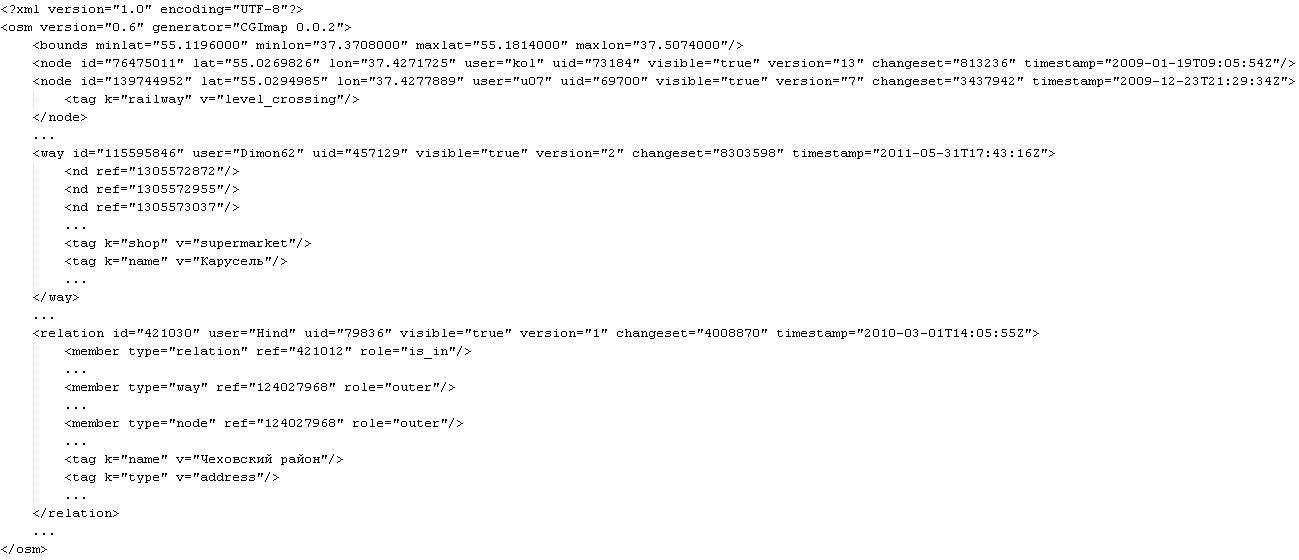
\includegraphics[width=1.1\linewidth]{example_osm}

Документ OSM состоит из двух основных частей: пролога и тела \linebreak
документа.

Как и обычный XML-документ пролог OSM-документа может \linebreak
содержать идентификационную информацию о нем или может быть\linebreak
абсолютно пустым.

В прологе документа обычно содержится объявление, \linebreak
указывающее на то, что это XML-документ, и содержащее номер \linebreak
версии (version) и используемую кодировку (encoding declaration):
\\[10pt]
<?xml version="1.0" encoding="UTF-8">
\\[10pt]
Второй основной частью OSM-документа является тело \linebreak
документа (Документ или корневой элемент), который в свою очередь \linebreak
содержит дополнительные элементы. К телу документа относится все, \linebreak
что заключено между тегами <osm> ... </osm>. Элементы, заключенные \linebreak
между этими тегами, несут в себе информацию, содержащуюся в \linebreak
документе (в нашем случае это информация о геообъектах, такая как\linebreak
тип объекта, его название, координаты и т.д.).

В OpenStreetMap нет ограничений на вводимые теги (так же как \linebreak
и для обычного XML-документа), но все же, как упоминалось ранее, для \linebreak
структурированной работы существует рекомендованный набор объектов и \linebreak
соответствующих им тегов. Основными такими тегами являются вложенные \linebreak
элементы <bounds/>, <node/>, <way/>, <relaition/>, <tag/>, а также \linebreak
некоторые другие, определеные в онотлогии к проекту.

Рассмотрим свойства основных тегов.

\begin{enumerate}
\item Элемент bounds. Включает в себя границы рассматриваемой области, \linebreak
которые определены атрибутами minlat, maxlat, minlon, maxlon.
\item Базовые элементы: точка (node), линия(way) и полигон(area).
\begin{itemize}
\item точка (node) - базовый элемент в структуре данных OSM. Точка \linebreak
имеет атрибуты 'широта' и 'долгота'. Точки используются для того, \linebreak
чтобы определить 'линию' (см. ниже), однако точка может являться\linebreak
и самостоятельным элементом карты, и использоваться для \linebreak
обозначения отдельного ни с чем не связанного объекта (например, \linebreak
телефонной будки, кафе, для указания координат, к которым \linebreak
привязано название населённого пункта или любого другого места. \linebreak
Отдельные точки (т.е. не входящие в состав линий или областей) \linebreak
всегда должны иметь хотя бы одно свойство.

Точки, входящие в состав линии, часто не имеют свойств и нужны \linebreak
только для описания линии; однако это не является незыблемым правилом.


\item линия (way). Линия представляет собой ломаную линию, \linebreak
проходящую через точки. Линия состоит, как минимум, из двух \linebreak
точек. Обычно линиями обозначаются улицы, дороги и т.д. Одна \linebreak
точка может принадлежать нескольким линиям одновременно.

Линия характеризуется свойствами, которые распространяются на \linebreak
неё на всём протяжении. Например, для линии, обозначающей \linebreak
дорогу, такими свойствами могут являться тип и качество покрытия, \linebreak
допустимая скорость движения и т.п. Если при уточнении \linebreak
выясняется, что не все свойства линии сохраняются на всём её \linebreak
протяжении (например, на дороге, которой соответствует линия, \linebreak
имеется участок с другим типом покрытия), то линия может быть \linebreak
разделена на части.

Для того, чтобы считаться корректно определённой, линия должна \linebreak
иметь хотя бы одно свойство.

\item полигон (area) или замкнутая линия (closed way) - элемент \linebreak
карты, предназначенный для описания участков поверхности. \linebreak
Полигон формируется замкнутой линией  (т.е. первая точка линии \linebreak
совпадает с последней) и является совокупностью этой самой \linebreak
линии и области, находящейся внутри контура этой линии. В этом \linebreak
смысле полигон не является самостоятельным типом элементов, \linebreak
а лишь псевдо-элементом, особой разновидностью линии с \linebreak
соответствующими свойствами.

Полигоны используются для обозначения участка поверхности, \linebreak
обладающего общими свойствами. Например, полигоны \linebreak
используются для описания водоёмов и лесов.

Корректно определённый полигон должен иметь хотя бы одно \linebreak
свойство.

Для описания вырезов, 'дыр' в полигонах, например, для описания \linebreak
участка занятого лесом, внутри которого имеется вырубленный \linebreak
участок рисуются мультиполигоны.
\end{itemize}
\item Элемент relation (отношение). Отношение группирует объекты по \linebreak
определенному признаку и для определенной цели. 'Участниками' \linebreak
(member) отношения могут любые объекты (точки, линии, области) и \linebreak
даже другие отношения. Эти элементы — участники отношения и \linebreak
каждому участнику присваивается 'роль' (role) в отношении. Как и \linebreak
другие типы элементов могут иметь теги. Один объект может \linebreak
входить в несколько отношений, а также несколько раз в одно и \linebreak
cто же отношение.

    Атрибут 'тип' (type) устанавливает разновидность отношения. \linebreak
    Отношения могут описывать замкнутые дороги, запреты поворотов и т.д.

    Расположение участников в отношении постоянно и определяется \linebreak
    очередностью добавления. Повторяющиеся объекты сохраняют их \linebreak
    определенный порядок.

\item Элемент tag (тег). Тег строго говоря не элемент, а свойство объекта. \linebreak
Каждый тег имеет атрибуты - ключ (k) и значение (v). Ключи и их \linebreak
значения описывают объект и наделяют его свойствами.
\end{enumerate}

Для всех элементов существуют общие атрибуты:

\begin{itemize}
\item user - имя пользователя, который совершал последнее изменение \linebreak
объекта;
\item uid - числовой идентификатор пользователя, который совершил \linebreak
последнее изменение объекта;
\item timestap - время последнего изменения;
\item visible - является ли объект удаленным в базе данных. Если visible='false', \linebreak
то объект должен быть возвращен вызовом истории изменений;
\item version - версия редакции объекта. Версия вновь созданных объектов \linebreak
равна 1, это значение увеличивается на сервере, когда клиент добавляет \linebreak
новую версию объекта. Сервер будет отклонять новую версию объекта, если \linebreak
версия присланная клиентом не соответствует текущей версии объекта в \linebreak
базе данных;
\item chengeset - пакет правок (история) в котором указаны создание и \linebreak
изменения объектов.
\end{itemize}

Особенности элемента 'точка'.

\begin{itemize}
\item атрибут id - числовой идентификационный номер, который уникален \linebreak
только среди точек. (Линия может иметь такое же id как и точка.);
\item атрибут lat - координаты широты;
\item атрибут lon - координаты долготы;
\item теги - множество пар тегов (ключ - значение) с уникальным ключом;
\end{itemize}

Особенности элемента 'линия'.

\begin{itemize}
\item атрибут id - числовой идентификационный номер, не являются \linebreak
уникальными, линия может иметь такой же идентификатор, как точка;
\item nodes - теги (nd) с атибутом ref (идентификатор точки), являющиеся \linebreak
списком всех точек идентификаторы которых составляют линию;
\item теги - множество пар тегов (ключ - значение) с уникальным ключом;
\end{itemize}

Особенности элемента 'отношение'.
\begin{itemize}
\item атрибут id - числовой идентификационный номер, не являются \linebreak
уникальными, линия может иметь такой же идентификатор, как точка;
\item теги - множество пар тегов (ключ - значение) с уникальным ключом;
\item members - упорядоченный список примитивов с атрибутами роль \linebreak
(где ролью может быть любой текст), тип (тип примитива), \linebreak
ref (идентификатор примитива).
\end{itemize}

\newpage
\subsection{XPath}
\subsubsection{Общие сведения}
Для получения необходимой информации из документа OSM в \linebreak
учебно-исследовательской работе используется язык XPath.

Язык XML Path (XPath) является набором синтаксических \linebreak
и семантических правил для ссылок на части XML-документов.\linebreak
XPath используется в URL для записи путей, обеспечивающих \linebreak
навигацию по иерархической структуре XML документа.

Главная задача языка XPath - адресация частей в XML документе. Для \linebreak
достижения этой цели язык дополнительно наделен основными функциями \linebreak
для манипулирования строками, числами и булевыми значениями. В XPath \linebreak
используется компактный синтаксис, отличающийся от принятого в XML \linebreak
и облегчающий использование языка XPath. XPath работает не с внешним \linebreak
синтаксисом XML документа, а с его абстрактной логической структурой. \linebreak
Язык XPath спроектирован так, что помимо поддержки адресации он \linebreak
обладает естественным набором элементов, которые могут использоваться \linebreak
для сравнения (проверки, соответствует ли узел некому шаблону).

XPath представляет XML-документ как дерево узлов. Узлы могут быть \linebreak
разных типов, таких как узлы элементов, узлы атрибутов или узлы \linebreak
текста. Для каждого типа узлов в XPath определяется способ вычисления \linebreak
строкового значения. Некоторые типы узлов имеют также имя. XPath \linebreak
полностью поддерживает пространства имен XML. В результате, имя любого \linebreak
узла в этом языке образуется из двух частей: локальной части и URI \linebreak
(унифицированный (единообразный) идентификатор ресурса - \linebreak
последовательность символов, идентифицирующая абстрактный или \linebreak
физический ресурс) некого пространства имен (возможно, нулевого). \linebreak
Такая комбинация называется расширенным именем.

Специальным типом узла является корневой узел. XML-документ \linebreak
содержит только один такой узел и он содержит весь XML-документ, \linebreak
т.е. корневой узел содержит корневой элемент, а также любые узлы \linebreak
инструкций обработки, объявлений или комментариев, которые \linebreak
появляются до или после корневого элемента.

Не существует типа узла для XML-декларации (такой, \linebreak
как <?xml version='1.0' encoding='UTF-8'?>). Следовательно, на \linebreak
такие сущности нельзя ссылаться в XPath.

Элементные узлы представляют каждый элемент в XML-документе. Узлы \linebreak
атрибутов принадлежат элементным узлам и представляют атрибуты. \linebreak
Однако, атрибуты, которые начинаются с xmlns: представляются в \linebreak
XPath с узлами пространств имен. Другие типы узлов включают в себя \linebreak
текстовые узлы, узлы инструкций обработки и узлы комментариев.

Главной синтаксической конструкцией языка XPath является выражение. \linebreak
В результате обработки выражения получается объект, относящийся к \linebreak
одному из четырех основных типов:

- набор узлов (node-set) - неупорядоченный набор узлов без дубликатов;

- булево значение (boolean) - true или false;

- число (number) - число с плавающей точкой;

- строка (string) - последовательность UCS символов.

\subsubsection{Типовые XPath-запросы}

Рассмотрим XPath-запросы на примере документа OSM:
\\[10pt]
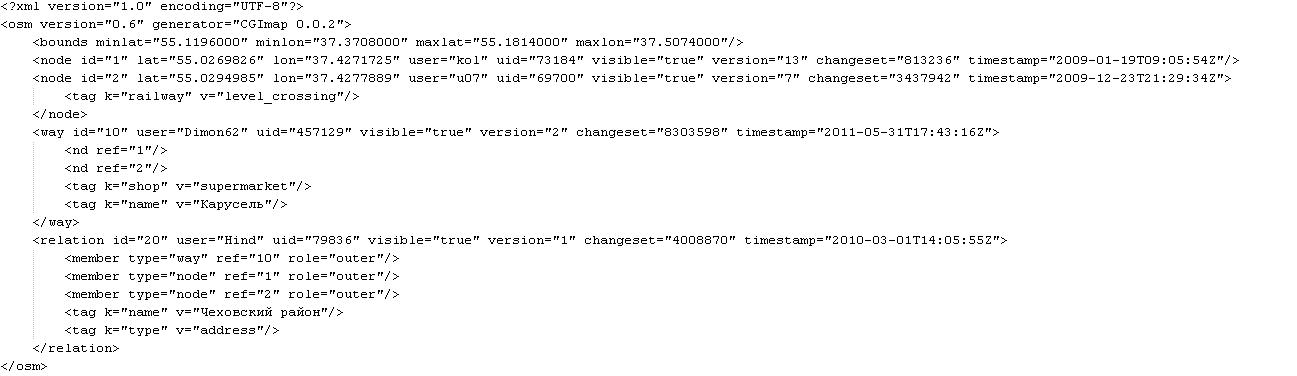
\includegraphics[width=1.15\linewidth]{examplemap_osm}

\textbf{Базовый синтаксис языка}

Базовый синтаксис языка XPath похож на адресацию в файловой системе. \linebreak
База языка - это оси. Оси служат для определения набора узлов \linebreak
относительно данного узла. В дополнение к базе существует набор функций, \linebreak
разделенных на 5 групп. Описание осей и функций находится в Приложении А. \linebreak
Основные оси языка XPath:
\begin{itemize}
\item attribute:: — возвращает множество атрибутов текущего элемента \linebreak
(можно заменить на '@');
\item child:: — возвращает множество потомков на один уровень ниже \linebreak
(часто просто опускают);
\item descendant:: — возвращает полное множество потомков (можно \linebreak
заменить на './/');
\item parent:: — возвращает предка на один уровень назад (можно \linebreak
заменить на '..');
\item self:: — возвращает текущий элемент (можно заменить на '.').
\end{itemize}

Если путь начинается с символа '/', то он представляет абсолютный путь \linebreak
к заданному элементу. Запрос '/osm' выберет корневой элемент \linebreak
<osm> ... </osm>. Этот запрос эквивалентен '/child::osm', но, как \linebreak
отмечалось ранее, подобная запись упрощается.
\vskip--10pt
'/osm/node/tag' - выбираются все элементы tag, являющиеся детьми \linebreak
элементов <node>, которые в свою очередь являются детьми корневого \linebreak
узла <osm>:
\vskip--10pt
<tag k='railway' v='level\_crossing'></tag>.
\vskip--10pt
Если путь начинается с //, то будут выбраны все элементы документа, \linebreak
которые соответствуют указанному шаблону, например, '//nd' - будут \linebreak
выбраны все элементы документа, соответствующие <nd>.
\vskip--10pt
<nd ref='1'></nd>

<nd ref='2'></nd>
\vskip--10pt
'//way/tag' - все элементы tag, являющиеся детьми <way>:
\vskip--10pt
<tag k='shop' v='supermarket'></tag>

<tag k='name' v='Карусель'></tag>
\vskip--10pt
Символ '*' указывает, что надо выбрать все элементы, соответствующие \linebreak
пути перед ней. Например, '/osm/node/*' - будут выбраны все элементы, \linebreak
являющиеся прямыми потомками /osm/node :
\vskip--10pt
<tag k='railway' v='level\_crossing'></tag>
\vskip--10pt
'/*/*/tag' - все элементы tag, имеющие двух предков.
\vskip--10pt
<tag k='railway' v='level\_crossing'></tag>

<tag k='shop' v='supermarket'></tag>

<tag k='name' v='Карусель'></tag>

<tag k='name' v='Чеховский район'></tag>

<tag k='type' v='address'></tag>

\vskip--10pt
'//*' - будут выбраны все возможные элементы.
\vskip--10pt

Выражение в квадратных скобках позволяет задавать более четкие \linebreak
критерии для элемента. Так число в квадратных скобках обозначает \linebreak
позицию элемента в выбранном множестве.
\vskip--10pt
'/osm/node[1]' - будет выбран первый потомок <node> элемента <osm>:
\vskip--10pt
<node id='1' lat='55.0269826' lon='37.4271725' user='kolen' ...>
\vskip--10pt

Несколько путей можно скомбинировать с помощью разделителя |.
\vskip--10pt
'//member | //bounds' - Выбираются все элементы member и bounds:
\vskip--10pt
<bounds minlat='55.1196000' minlon='37.3708000' ...></bounds>

<member type='way' ref='10' role='admin\_centre'></member>

<member type='node' ref='1' role='outer'></member>

<member type='node' ref='2' role='outer'></member>
\vskip--10pt
'//tag[@v]' - выбираются элементы tag, имеющие атрибут '@v' \linebreak
(может быть также записан как '//tag[attribute::v]):
\vskip--10pt
<tag k='railway' v="level\_crossing"></tag>

<tag k='shop' v='supermarket'></tag>

<tag k='name' v='Карусель'></tag>

<tag k='name' v='Чеховский район'></tag>

<tag k='type' v='address'></tag>
\vskip--10pt
Ось descendant содержит потомков контекстного узла; потомком является \linebreak
дочерний элемент, дочерний элемент дочернего элемента и так далее; \linebreak
таким образом ось descendant не содержит узлов атрибутов и \linebreak
пространств имен.
\vskip--10pt
'//node/descendant::tag' - выбираются элементы tag, имеющие в качестве \linebreak
предка элемент node:
\vskip--10pt
<tag k='railway' v='level\_crossing'/>
\vskip--10pt
Ось parent содержит родителя контекстного узла, если он существует:
\vskip--10pt
'//bounds/parent::*' - результат:
\vskip--10pt
 <osm version='0.6' generator='CGImap 0.0.2'></osm>;
\vskip--10pt

\newpage
\subsection{PostgreSQL и OpenGIS}
\subsubsection{PostgreSQL}
Геоданные предполагается хранить в базе данных.

База данных (БД) - это поименнованная совокупность \linebreak
структурированных данных, относящихся к определенной предметной \linebreak
области.

Для создания баз данных, поддержания их в актуальном состоянии \linebreak
и организации поиска в них необходимой информации используется \linebreak
комплекс программных и языковых средств - система управления \linebreak
базами данных (СУБД). СУБД позволяют структурировать, \linebreak
систематизировать и организовывать данные для их компьютерного \linebreak
хранения и обработки.

Основные функции СУБД:

\begin{itemize}
\item физическое размещение в памяти данных и их описаний;
\item реализация механизмов поиска запрашиваемых данных;
\item решение проблем, возникающих при одновременном запросе одних и тех \linebreak
же данных многими пользователями (прикладными программами);
\item обеспечение защиты данных от некорректных обновлений и (или) \linebreak
    несанкционированного доступа;
\item поддержание баз данных в актуальном состоянии;
\item обеспечение целостности и непротиворечивости данных.
\end{itemize}

СУБД различаются по типу используемых моделей данных, а также по способу доступа к базе данных.

По типу используемых моделей данных СУБД различают как:
\begin{itemize}
\item иерархические;
\item сетевые;
\item реляционные;
\item объектно-ориентированные;
\item объектно-реляционные.
\end{itemize}

\begin{enumerate}
\item Иерархические СУБД (например, Information Management System (IMS)) \linebreak
- поддерживают древовидную организацию информации. Связи между записями \linebreak
выражаются в виде отношений предок/потомок, а у каждой записи есть \linebreak
ровно одна родительская запись. Это помогает поддерживать ссылочную \linebreak
целостность. Когда запись удаляется из дерева, все ее потомки также \linebreak
должны быть удалены.

Иерархические базы данных имеют централизованную структуру, \linebreak
т.е. безопасность данных легко контролировать. Поиск записи \linebreak
осуществляется методом прямого обхода дерева. Отсюда следует \linebreak
необходимость правильно упорядочивать записи, чтобы время их \linebreak
поиска было минимальным. Это трудно, так как не все отношения, \linebreak
существующие в реальном мире, можно выразить в иерархической \linebreak
базе данных. Отношения 'один ко многим' являются естественными, \linebreak
но практически невозможно описать отношения 'многие ко многим' \linebreak
или ситуации, когда запись имеет несколько предков.

\item Сетевые СУБД (например, Integrated Database Management \linebreak
System (IDMS)). Сетевая модель расширяет иерархическую модель СУБД, \linebreak
позволяя группировать связи между записями в множества. С \linebreak
логической точки зрения связь — это не сама запись. Связи лишь \linebreak
выражают отношения между записями. В сетевой модели допускаются \linebreak
отношения 'многие ко многим', а записи не зависят друг от \linebreak
друга. При удалении записи удаляются и все ее связи, но не сами \linebreak
связанные записи.

В сетевой модели требуется, чтобы связи устанавливались между \linebreak
существующими записями во избежание дублирования и искажения \linebreak
целостности. Данные можно изолировать в соответствующих таблицах \linebreak
и связать с записями в других таблицах.

Программисту не нужно, при проектировании СУБД, заботиться о том, \linebreak
как организуется физическое хранение данных на диске. Это \linebreak
ослабляет зависимость приложений и данных. Но в сетевой модели \linebreak
требуется, чтобы программист помнил структуру данных при \linebreak
формировании запросов.

\item Реляционные СУБД (например, System R, Ingres). В сравнении \linebreak
с рассмотренными выше моделями реляционная модель требует от \linebreak
сервера СУБД гораздо более высокого уровня сложности. В ней делается \linebreak
попытка избавить программиста от выполнения рутинных операций по \linebreak
управлению данными, характерных для иерархической и сетевой моделей.

В реляционной модели база данных представляет собой \linebreak
централизованное хранилище таблиц, обеспечивающее безопасный \linebreak
одновременный доступ к информации со стороны многих \linebreak
пользователей. В строках таблиц часть полей содержит данные, \linebreak
относящиеся непосредственно к записи, а часть — ссылки на \linebreak
записи других таблиц. Таким образом, связи между записями \linebreak
являются неотъемлемым свойством реляционной модели. Каждая \linebreak
запись таблицы имеет одинаковую структуру.

В реляционной модели СУБД достигается информационная и \linebreak
структурная независимость. Записи не связаны между собой \linebreak
настолько, чтобы изменение одной из них затронуло остальные.

В реляционных СУБД применяется язык SQL, позволяющий \linebreak
формулировать произвольные, нерегламентированные запросы. \linebreak
Реляционные базы данных страдают от различий в реализации \linebreak
языка SQL, хотя это и не проблема реляционной модели. Каждая \linebreak
реляционная СУБД реализует какое-то подмножество стандарта \linebreak
SQL плюс набор уникальных команд, что усложняет задачу \linebreak
программистам, пытающимся перейти от одной СУБД к другой.

\item Объектно-ориентированные СУБД (O2, ORION, Iris). Позволяют \linebreak
программистам интерпретировать все свои информационные сущности \linebreak
как объекты, хранящиеся в оперативной памяти. Дополнительный \linebreak
интерфейсный уровень абстракции обеспечивает перехват запросов, \linebreak
обращающихся к тем частям базы данных, которые находятся в \linebreak
постоянном хранилище на диске. Изменения, вносимые в объекты, \linebreak
оптимальным образом переносятся из памяти на диск.

Преимуществом ООСУБД является упрощенный код. Приложения \linebreak
получают возможность интерпретировать данные в контексте того \linebreak
языка программирования, на котором они написаны. Реляционная \linebreak
база данных возвращает значения всех полей в текстовом виде, а \linebreak
затем они приводятся к локальным типам данных. В ООБД этот этап \linebreak
ликвидирован. Методы манипулирования данными всегда остаются \linebreak
одинаковыми независимо от того, находятся данные на диске или \linebreak
в памяти.

С помощью ООСУБД решаются две проблемы. Во-первых, сложные \linebreak
информационные структуры выражаются в них лучше, чем в \linebreak
реляционных базах данных, а во вторых, устраняется \linebreak
необходимость транслировать данные из того формата, \linebreak
который поддерживается в СУБД.

В объектной модели данных поддерживаются нерегламентированные \linebreak
запросы, но языком их составления не обязательно является SQL. \linebreak
Логическое представление данных может не соответствовать \linebreak
реляционной модели, поэтому применение языка SQL станет \linebreak
бессмысленным. Зачастую удобнее обрабатывать объекты в памяти, \linebreak
выполняя соответствующие виды поиска.

Большим недостатком объектно-ориентированных баз данных является \linebreak
их тесная связь с применяемым языком программирования. К данным, \linebreak
хранящимся в реляционной СУБД, могут обращаться любые \linebreak
приложения, тогда как, к примеру, Java-объект, помещенный \linebreak
в ООСУБД, будет представлять интерес лишь для приложений, \linebreak
написанных на Java.

\item Объектно-реляционные СУБД (PostgreSQL). Объединяют в себе черты \linebreak
реляционной и объектной моделей. Их возникновение объясняется тем, \linebreak
что реляционные базы данных хорошо работают со встроенными типами \linebreak
данных и гораздо хуже — с пользовательскими, нестандартными. \linebreak
Когда появляется новый важный тип данных, приходится либо включать \linebreak
его поддержку в СУБД, либо заставлять программиста \linebreak
самостоятельно управлять данными в приложении.

Объектно-реляционная СУБД позволяет загружать код, \linebreak
предназначенный для обработки 'нетипичных' данных. \linebreak
Таким образом, база данных сохраняет свою табличную структуру, \linebreak
но способ обработки некоторых полей таблиц определяется извне, \linebreak
т.е. программистом.
\end{enumerate}

По способу доступа к базе данных СУБД различаются как:
\begin{enumerate}
\item  Файл-серверные СУБД. В файл-серверных СУБД файлы данных \linebreak
располагаются централизованно на файл-сервере СУБД. Ядро СУБД \linebreak
располагается на каждом клиентском компьютере. Доступ к данным \linebreak
осуществляется через локальную сеть. Синхронизация чтений и \linebreak
обновлений осуществляется посредством файловых блокировок. \linebreak
Преимуществом этой архитектуры является низкая нагрузка на \linebreak
ценральный процессор сервера, а недостатком — высокая загрузка \linebreak
локальной сети.

\item Клиент-серверные СУБД. Такие СУБД состоят из клиентской части \linebreak
(которая входит в состав прикладной программы) и сервера СУБД. \linebreak
Клиент-серверные СУБД, в отличие от файл-серверных, обеспечивают \linebreak
разграничение доступа между пользователями и мало загружают сеть \linebreak
и клиентские машины. Сервер является внешней по отношению к \linebreak
клиенту программой, и по надобности его можно заменить другим. \linebreak
Недостаток клиент-серверных СУБД в самом факте существования \linebreak
сервера СУБД (что плохо для локальных программ — в них удобнее \linebreak
встраиваемые СУБД) и больших вычислительных ресурсах, потребляемых сервером.

\item Встраиваемые СУБД. Встраиваемая СУБД — библиотека, которая \linebreak
позволяет унифицированным образом хранить большие объёмы данных \linebreak
на локальной машине. Доступ к данным может происходить через SQL \linebreak
либо через особые функции СУБД. Встраиваемые СУБД быстрее \linebreak
обычных клиент-серверных и не требуют установки сервера, \linebreak
поэтому востребованы в локальном ПО, которое имеет дело с \linebreak
большими объёмами данных.
\end{enumerate}

В учебно-исследовательской работе использована свободная \linebreak
объектно-реляционная клиент-серверная СУБД PostgreSQL.

История PostgreSQL начинается с 1977 года с \linebreak
разработки в Калифорнийском университете Беркли базы данных Ingres. \linebreak
В 1996 был открыт исходный код PostgreSQL для программистов, и \linebreak
началось её развитие под девизом Open Source. Данная СУБД \linebreak
была выбрана для проекта не только из-за того, что она \linebreak
является открытой. PostgreSQL выбрана из-за того, что в \linebreak
распоряжении PostgreSQL есть расширение PostGIS, осуществляющее \linebreak
поддержку хранения геоданных в соответствии со стандартом \linebreak
хранения геоданных OpenGis.

\newpage
\subsubsection{Стандарт OpenGIS}

Хранение геоданных — одна из самых актуальных задач в области хранения \linebreak
данных. Будь то каталог автозаправок, база данных городов, система \linebreak
отслеживания пробок — везде требуется эффективная система хранения \linebreak
больших объемов географических данных.

За стандартизацию этой области на данный момент отвечает \linebreak
Open Geospatial Consortium (OGC) или сокращенно Open GIS, в который \linebreak
входит более 370 организаций. В течение нескольких лет были \linebreak
составлены 28 стандартов.

OpenGIS даёт следующие преимущества:

\begin{itemize}
\item позволяет хранить геометрический/географический объект в виде \linebreak
одного кортежа и строить реляционные связи между этими объектами \linebreak
и другими данными БД;
\item позволяет строить индексы по геометрическим полям и выполнять \linebreak
выборки с их помощью;
\item предоставляет набор функций для манипулирования и выявления \linebreak
отношений между объектами (включение, пересечение, расстояние, \linebreak
соприкасание и т.п.);
\end{itemize}

Все разработчики СУБД стремятся создавать расширения для работы \linebreak
с геоданными в соответствии со стандартами OpenGIS. Как отмечалось \linebreak
ранее у PosgreSQL существует расширение - PostGIS, позволяющее \linebreak
этой СУБД хранить геоданные в соответствии со стандартами OpenGIS.

Спецификация OpenGIS определяет стандартные типы объектов ГИС, \linebreak
функции для манипуляции ими, и набор таблиц метаданных. В целях \linebreak
сохранения корректности метаданных, такие операции как создание \linebreak
и удаление столбцов с пространственными данными осуществляются \linebreak
с помощью специальных процедур, определенных OpenGIS.

Спецификация OpenGIS определяет два стандартных способа \linebreak
определения пространственных объектов: в форме Well-Known Text \linebreak
(WKT) и в форме Well-Known Binary (WKB). WKT и WKB включают \linebreak
информацию о типе объекта и координаты, составляющие объект.

Примеры текстового представления (WKT) пространственных \linebreak
объектов приведены ниже:

-- POINT(0 0)

-- LINESTRING(0 0,1 1,1 2)

-- POLYGON((0 0,4 0,4 4,0 4,0 0),(1 1, 2 1, 2 2, 1 2,1 1))

-- MULTIPOINT(0 0,1 2)

-- MULTILINESTRING((0 0,1 1,1 2),(2 3,3 2,5 4))

-- MULTIPOLYGON(((0 0,4 0,4 4,0 4,0 0),(1 1,2 1,2 2,1 2,1 1)), \linebreak
((-1 -1,-1 -2,-2 -2,-2 -1,-1 -1)))

-- GEOMETRYCOLLECTION(POINT(2 3),LINESTRING((2 3,3 4)))

Кроме того, стандартом OpenGIS определены две таблицы метаданных: \linebreak
SPATIAL\_REF\_SYS и GEOMETRY\_COLUMNS. Эти две таблицы и \linebreak
обеспечивают поддержку стандарта OpenGIS для PostGIS.

Таблица SPATIAL\_REF\_SYS содержит числовые идентификаторы и \linebreak
текстовые описания систем координат, используемых в \linebreak
пространственной базе данных, и определяется следующим образом:
\\[10pt]
CREATE TABLE spatial\_ref\_sys (

	srid       INTEGER NOT NULL PRIMARY KEY,

	auth\_name  VARCHAR(256),

	auth\_srid  INTEGER,

	srtext     VARCHAR(2048),

	proj4text  VARCHAR(2048)

)
\\[10pt]
В этой таблице столбец srid - уникальный идентификатор \linebreak
пространственной системы координат (Spatial Referencing System, SRS) \linebreak
в пределах этой таблицы. SRID представляет из себя числовой код, \linebreak
которому соответствует некоторая система координат. Например, \linebreak
распространенный код EPSG 4326 соответствует географической системе координат WGS84.

Колонка auth\_name содержит название стандарта или \linebreak
стандартизирующего органа, на который ссылается данная справочная \linebreak
система. Например, EPSG будет правильным значением для auth\_name.

Столбец auth\_srid - идентификатор пространственной системы \linebreak
координат, указанной в auth\_name. В случае EPSG, это должен \linebreak
быть код проекции EPSG.

Srtext содержит в себе WNT (well-known text) представление системы \linebreak
координат.

PostGIS использует библиотеку Proj4 для преобразований систем \linebreak
координат. Столбец proj4text содержит строковое определение \linebreak
координат Proj4 для данного SRID.

Таблица GEOMETRY\_COLUMNS хранит информацию о таблицах базы \linebreak
данных, содержащих пространственную информацию и определяется \linebreak
следующим образом:
\\[10pt]
CREATE TABLE geometry\_columns (

	f\_table\_catalog    VARCHAR(256) NOT NULL,

	f\_table\_schema     VARCHAR(256) NOT NULL,

	f\_table\_name       VARCHAR(256) NOT NULL,

	f\_geometry\_column  VARCHAR(256) NOT NULL,

	coord\_dimension    INTEGER NOT NULL,

	srid               INTEGER NOT NULL,

	type               VARCHAR(30) NOT NULL

)
\\[10pt]
Здесь столбцы f\_table\_catalog, f\_table\_schema, f\_table\_name содержат \linebreak
в себе все составляющие имени таблицы с геометрическим столбцом, \linebreak
аналогично Oracle. В PosgreSQL нет аналога понятия 'каталог', поэтому \linebreak
эта колонка всегда пуста. В колонке 'схема' хранится имя схемы в \linebreak
PostgreSQL (по умолчанию всегда 'public').

Столбец f\_geometry\_column содержит имя геометрического столбца в \linebreak
основной таблице.

В колонке coord\_dimension указывается геометрическая размерность \linebreak
столбца (2, 3, 4-мерное измерение).

Srid - внешний ключ на таблицу SPATIAL\_REF\_SYS, содержит \linebreak
идентификаторы пространственной справочной системы, используемой \linebreak
для координатной геометрии в указанной таблице.

Колонка type содержит типы пространственных объектов. \linebreak
Ограничивает пространственный столбец единственным типом, одним \linebreak
из следующих: POINT, LINESTRING, POLYGON, MULTIPOINT, \linebreak
MULTILINESTRING, MULTIPOLYGON, GEOMETRYCOLLECTION \linebreak
(или POINTM, соответствующим XYM-версиям), LINESTRINGM, \linebreak
POLYGONM, MULTIPOINTM, MULTILINESTRINGM, MULTIPOLYGONM, \linebreak
GEOMETRYCOLLECTIONM. Для разнородных (смешанный тип) \linebreak
коллекций возможно использование 'GEOMETRY' как типа. \linebreak
Этот атрибут не является частью спецификации OpenGIS, но он \linebreak
необходим для обеспечения типового единообразия.

Заполнение этой таблицы осуществляется вручную, либо с помощью \linebreak
специальной процедуры OGC AddGeometryColumn().


\newpage
\subsection{SQL}
Для помещения информации о геообъектах в базу данных использован \linebreak
язык SQL. В данной главе описывается структура и синтаксис языка \linebreak
SQL, а также приведены типовые SQL-запросы и пространственные запросы.

\subsubsection{Общие сведения}
Язык SQL (Structured Query Language - структурированный язык запросов) \linebreak
представляет собой стандартный высокоуровневый язык описания данных и \linebreak
манипулирования ими в системах управления базами данных (СУБД), \linebreak
построенных на основе реляционной модели данных.

Язык SQL разработан фирмой IBM в конце 70-х годов. Первый \linebreak
международный стандарт языка принят международной \linebreak
стандартизирующей организацией ISO в 1989 году, а новый \linebreak
(более полный) - в 1992 году. Официальное название стандарта - \linebreak
Международный стандарт языка баз данных SQL (1992) \linebreak
(International Standart Database Language SQL), неофициальное \linebreak
название - SQL/92, или SQL-92, или SQL92. Язык SQL стал \linebreak
фактически стандартным языком доступа к базам данных. Все \linebreak
производители реляционных СУБД поддерживают с различной степенью \linebreak
соответствия стандарт SQL92.

Язык SQL представляет собой совокупность операторов, инструкций \linebreak
и вычисляемых функций.

Основу языка SQL составляют операторы, условно разбитые не несколько \linebreak
групп по выполняемым функциям.

Можно выделить следующие группы операторов:

\begin{enumerate}
\item Операторы DDL (Data Definition Language) - операторы определения и \linebreak
    манипулирования схемой базы данных (CREATE, DROP, ALTER).

    CREATE создает объект БД (саму базу, таблицу, представление, \linebreak
    пользователя и т. д.);

    ALTER изменяет объект;

    DROP удаляет объект.

\item Операторы DML (Data Manipulation Language) - операторы \linebreak
манипулирования данными (SELECT, INSERT, DELETE, UPDATE).

    SELECT считывает данные, удовлетворяющие заданным условиям;

    INSERT добавляет новые данные;

    UPDATE изменяет существующие данные;

    DELETE удаляет данные.

\item DCD (Data Control Language)- операторы защиты и управления данными \linebreak
(GRANT, REVOKE).

    GRANT предоставляет пользователю (группе) разрешения на \linebreak
    определенные операции с объектом;

    REVOKE отзывает ранее выданные разрешения;

    DENY задает запрет, имеющий приоритет над разрешением.
\end{enumerate}

\subsubsection{Типовые SQL-запросы}

SQL-запрос состоит из ключевых слов и слов, определяемых пользователем. \linebreak
Ключевые слова являются постоянной частью языка SQL и имеют \linebreak
фиксированное значение. Их следует записывать в точности так, как это \linebreak
установлено, нельзя разбивать на части для переноса с одной строки \linebreak
на другую. Слова, определяемые пользователем, задаются им самим \linebreak
(в соответствии с синтаксическими правилами) и представляют собой \linebreak
идентификаторы или имена различных объектов БД. Слова в запросе \linebreak
размещаются также в соответствии с установленными синтаксическими \linebreak
правилами.

Каждый запрос начинается с глагола, т.е. ключевого слова, \linebreak
описывающего выполняемое действие, и заканчивается точкой \linebreak
с запятой (SELECT, CREATE, INSERT, DELETE и т.д.)

После глагола следует одно или несколько предложений. Они описывают \linebreak
данные, с которыми работает запрос, или содержат уточняющую \linebreak
информацию о действии, выполняемом запросом. Каждое \linebreak
предложение начинается с ключевого слова, например WHERE (где), \linebreak
FROM (откуда), INTO (куда) и HAVING(имеющий). Одни предложения \linebreak
в запросе могут изменяться, а другие - нет. При этом конкретная \linebreak
структура и содержимое предложения также могут изменяться. \linebreak
Многие предложения содержат имена таблиц или столбцов; \linebreak
некоторые из них могут содержать дополнительные ключевые слова, \linebreak
константы и выражения.

Глаголы, с которых начинаются запросы, и ключевые слова (слова, \linebreak
которые в SQL зарезервированы для специального использования и \linebreak
являются частью его синтаксиса) записываются заглавными буквами, \linebreak
чтобы отличать их от имен столбцов и таблиц. Но в общем случае \linebreak
синтаксис SQL-запросов не чувствителен к расположению текста \linebreak
по строкам и к регистру символов.

Чтобы получить информацию, хранящуюся в базе данных используется \linebreak
запрос \textbf{SELECT}. Базовое действие этого запроса ограничено \linebreak
одной таблицей, хотя существуют конструкции, обеспечивающие \linebreak
выборку с нескольких таблиц одновременно. Для того, чтобы \linebreak
получить все строки данных для специфических столбцов, используется \linebreak
запрос такого вида:
\vskip--10pt
SELECT column1, column2 FROM table\_name;
\vskip--10pt
Также, можно получить все столбцы из таблицы, используя \linebreak
подстановочный знак «*»:
\vskip--10pt
SELECT * FROM table\_name;
\vskip--10pt
Это может быть полезно в том случае, когда необходимо выбрать данные \linebreak
с определенным условием WHERE. Следующий запрос возвратит все \linebreak
столбцы со всех строк, где «column1» содержит значение «3»:
\vskip--10pt
SELECT * FROM table\_name WHERE column1=3;
\vskip--10pt
Кроме «=» (равно), существуют следующие условные операторы:
\begin{itemize}
\item =	равно;
\item <>	не равно;
\item >	больше;
\item <	меньше;
\item >=	больше или равно;
\item <=	меньше или равно;
\end{itemize}

Запрос \textbf{INSERT} используется для создания новой строки данных. \linebreak
Для обновления уже существующих данных или пустых полей строки \linebreak
нужно использовать запрос UPDATE.

Примерный синтаксис запроса INSERT:
\vskip--10pt
INSERT INTO table\_name (column1, column2, column3) VALUES (‘data1’, ‘data2’, ‘data3’);
\vskip--10pt
Если предполагается вставлять все значения в порядке, в котором \linebreak
находятся столбцы таблицы, то можно и не указывать имена столбцов, \linebreak
хотя для удобочитаемости это предпочтительнее. Кроме того, если  \linebreak
столбцы перечисляются, то необязательно указывать их по порядку \linebreak
нахождения в базе данных, пока вводимые значения, соответствуют \linebreak
этому порядку. Не нужно перечислять столбцы, в которые не вводится \linebreak
информация.

Изменяется уже существующая информация в базе данных очень похожим \linebreak
образом.

\textbf{UPDATE} используется для того, чтобы изменить существующие \linebreak
значения или освободить поле в строке, поэтому новые значения \linebreak
должны соответствовать существующему типу данных и обеспечивать \linebreak
приемлемые значения. Если нужно изменить значения не во всех \linebreak
строках, то нужно использовать условие WHERE.
\vskip--10pt
UPDATE table\_name SET column1 = ‘data1’, column2 = ‘data2’ \linebreak
WHERE column3 = ‘data3’;
\vskip--10pt
Можно использовать WHERE для любого столбца, включая тот, \linebreak
который необходимо изменить. Это используется когда необходимо \linebreak
заменить одно определенное значение на другое.
\vskip--10pt
UPDATE table\_name SET FirstName = ‘Василий’ \linebreak
WHERE FirstName = ‘Василий’ AND LastName = ‘Сидоров’;
\vskip--10pt

Запрос \textbf{DELETE} полностью удаляет строку из базы данных. Если \linebreak
необходимо удалить одно единственное поле, то нужно использовать \linebreak
запрос UPDATE и установить для этого поля значение, которое \linebreak
будет являться аналогом NULL в программе. Необходимо \linebreak
ограничивать запрос DELETE условием WHERE, иначе  можно потерять \linebreak
все содержимое таблицы.
\vskip--10pt
DELETE FROM table\_name WHERE column1 = ‘data1’;
\vskip--10pt
Как только строка была удалена из базы данных, она не подлежит \linebreak
восстановлению.

\newpage
\subsection{Язык C++ и библиотека QT}

Функциональность модуля реализована с помощью языка С++ и \linebreak
библиотеки Qt.

Язык C++ — компилируемый статически типизированный язык \linebreak
программирования общего назначения. Сочетает в себе свойства \linebreak
как высокоуровневых, так и низкоуровневых языков за счет поддержки \linebreak
разных парадигм программирования.

Являясь одним из самых популярных языков программирования, \linebreak
C++ широко используется для разработки программного обеспечения. \linebreak
Область его применения включает создание операционных систем, \linebreak
разнообразных прикладных программ, драйверов устройств, приложений \linebreak
для встраиваемых систем, высокопроизводительных серверов, а также \linebreak
развлекательных приложений (например, видеоигры).

Стандарт C++ на 2003 год состоит из двух основных частей: описание \linebreak
ядра языка и описание стандартной библиотеки. Кроме того, существует \linebreak
огромное количество библиотек C++, не входящих в стандарт. \linebreak
Одной из таких библиотек является библиотека Qt.

Библиотека Qt - инструментарий для быстрой разработки графических \linebreak
интерфейсов (GUI) приложений на языке C++, с целью упростить \linebreak
перенос GUI-приложений с одной платформы на другую, т.е. такие \linebreak
приложения должны работать и в среде Windows, и в среде Unix/Linux \linebreak
под X11, и на компьютерах Macintosh одинаково.

В настоящее время Qt предоставляет использующему её программисту \linebreak
целостный фреймворк (framework), позволяющий при написании \linebreak
большей части приложения использовать только 'родные' классы Qt \linebreak
и практически полностью отказаться от написания системно-зависимого \linebreak
кода, использования системных вызовов или от изобретения \linebreak
собственных кросс-платформенных обёрток. Классы Qt удовлетворяют \linebreak
почти всем потребностям программиста. В Qt предусмотрены классы и \linebreak
для работы со строками, и для работы с файлами, сетью, базами \linebreak
данных, XML, и для обеспечения многопоточности в приложении, и \linebreak
многое-многое другое.

%К: теоретическая часть
%Н: описание алгоритма
\newpage
\section{Описание алгоритма работы модуля}
\subsection{Описание логики алгоритма}
Алгоритм включает в себя следующие этапы:
\begin{enumerate}
\item Выбор файла OpenStreetMap в формате OSM, в котором \linebreak
содержится необходимая информация.

Выбор файла OSM осуществляется пользователем с помощью \linebreak
диалогового окна из конфигурационного файла.

\item Формирование запроса к OSM-файлу для извлечения геоданных \linebreak
об объектах необходимого типа.

Формирование запроса происходит без участия пользователя. \linebreak
Для него этот процесс скрыт.

\item Формирование результата запроса, вывод извлеченных геоданных на экран.

Результаты запроса выводятся на экран в соответствующем окне программы.

\item Формирование SQL-запроса к базе данных для сохранения извлеченных \linebreak
геоданных в формате OpenGIS.

SQL-запрос формируется до запуска модуля. Формируется без участия \linebreak
пользователя.

\item Формирование отчёта о занесении геоданных в базу данных.

Отчёт о занесении геоданных в БД выводится на экран в соответствующем \linebreak
окне программы.

\item Графическое представление извлеченных геоданных.

В соответствующем окне программы представляется графическое \linebreak
изображение полученных геоданных.

\end{enumerate}

\newpage
\subsection{Блок-схема алгоритма}

\begin{figure}[h!]
\center{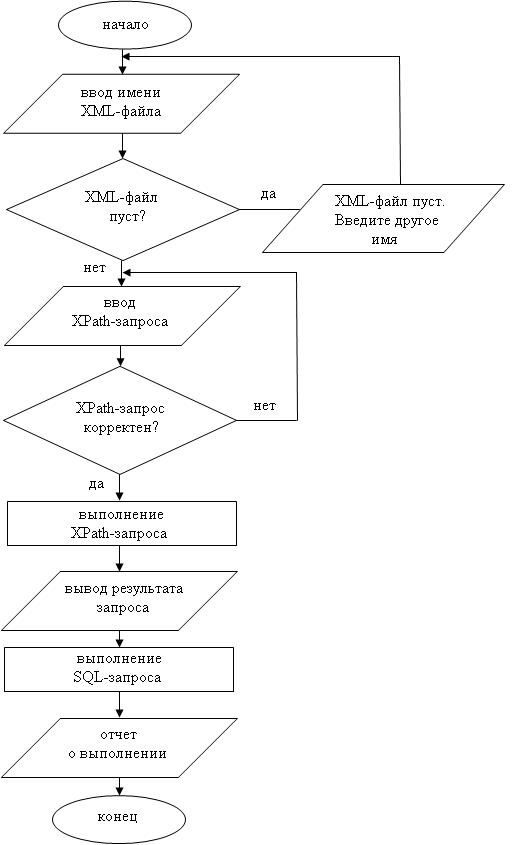
\includegraphics[width=0.9\linewidth]{box}}
\end{figure}
%К: описание алгоритма
%Н: практическая часть
\newpage
\section{Практическая часть}
\subsection{Фрагменты программного кода}

В этом разделе описаны основные XPath-выражения и SQL-запросы, \linebreak
задействованные в решении поставленной задачи, а также структура \linebreak
базы данных. Программный код модуля приведен в Приложении B.

\subsubsection{Используемые XPath-выражения}

Рассмотрим документ OSM XML:
\\[10pt]
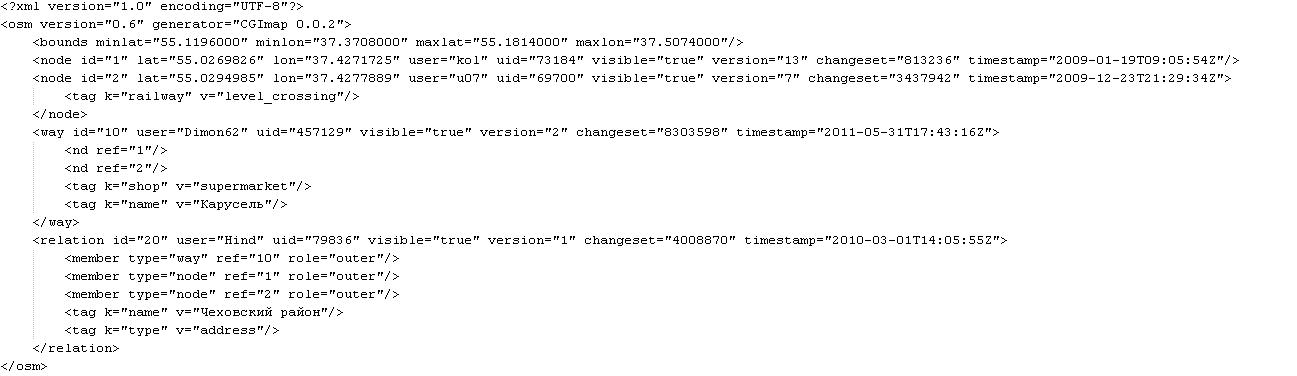
\includegraphics[width=1.15\linewidth]{examplemap_osm}
\\[10pt]
Для извлечения координат границ рассматриваемой области используется \linebreak
XPath-запрос следующего вида:
\vskip--10pt
'/osm/bounds/@minlat' - минимальная широта, результат minlat='55.1196000'

'/osm/bounds/@minlon' - минимальная долгота, результат minlon='37.3708000';

'/osm/bounds/@maxlat' - максимальная широта, результат maxlat='55.1814000';

'/osm/bounds/@maxlon' - максимальная долгота, результат maxlon='37.5074000'.
\vskip--10pt
Для извлечения всех названий типа node (точка) и way (линия), \linebreak
используется XPath-запросы:
\vskip--10pt
'/osm/way[*/@k='name']/@id' - результат: id='10';
\vskip--10pt
Для получения широты и долготы точки используется запрос:
\vskip--10pt
'/osm/node[@id='1']/@lat' - результат: lat='55.0269826'. \linebreak
Для долготы аналогично.
\vskip--10pt
Остальные запросы представляют из себя комбинацию тех или иных \linebreak
запросов, уже описанных в этой главе и главе, посвященной XPath-запросам.

\subsubsection{Структура базы данных}

Для решения поставленной задачи создана пространственная база данных, \linebreak
включающая в себя таблицы GEOMETRY\_COLUMNS и SPATIAL\_REF\_SYS. \linebreak
Кроме этого в базе данных созданы таблицы objects и tags, \linebreak
которые нужны непосредственно для хранения извлеченных геоданных.

Таблица objects хранит идентификаторы объектов и непосредственно \linebreak
сами объекты. Определяется следующим образом:
\vskip--10pt
CREATE TABLE objests (

	id\_obj        INTEGER NOT NULL,

  geometry\_obj  GEOMETRY,

)
\vskip--10pt
Колонка id\_obj содержит идентификаторы объектов.

Колонка geometry\_obj является геометрическим столбцом. Объект \linebreak
может иметь один из указанных ранее типов, например, POINT, \linebreak
LINESTRING, POLYGON, MULTIPOINT, MULTILINESTRING, \linebreak
MULTIPOLYGON и т.д.

Таблица tags хранит в себе имя и тип тегов, относящихся к определенному \linebreak
объекту из таблицы objects, определяется следующим образом:
\vskip--10pt
CREATE TABLE tags(

id\_tag integer NOT NULL,

key\_tag character varying(50),

value\_tag character varying(50),

id\_obj integer NOT NULL

)
\vskip--10pt
Колонка id\_tag содержит идентификаторы тегов.

Колонка key\_tag включает тип тега (или название характеристики, \linebreak
или атрибута объекта) в том виде, в котором они представлены в \linebreak
XML-документе, например 'name', 'building', 'street' и т.д.

Value\_tag содержит значения характристик (или атриутов, типов) \linebreak
объекта, например, у объекта с атрибутом 'name' может быть \linebreak
значение 'Московская область', у 'street' - 'Улица Гагарина', и т.д.

Колонка id\_obj хранит в себе внешний ключ на таблицу objects, \linebreak
содержит идентификаторы объектов.

\subsubsection{Используемые SQL-выражения}

Основные SQL-запросы, использующиеся для решения поставленной задачи.

Во-первых, это запросы с использованием операторов DDL. В ходе работы \linebreak
созданы 4 таблицы: objects, tags, GEOMETRY\_COLUMNS и \linebreak
SPATIAL\_REF\_SYS. Запрос создания таблицы objects с атрибутами \linebreak
id\_obj и name\_obj выглядит так:
\vskip--10pt
CREATE TABLE objects (

	id\_obj       INTEGER NOT NULL,

	name\_obj     VARCHAR(50),

	CONSTRAINT tag\_pkey PRIMARY KEY (id\_obj)

);
\vskip--10pt
Запрос создания таблицы tags:
\vskip--10pt
CREATE TABLE tags (

	id\_tag integer NOT NULL,

  key\_tag character varying(50),

  value\_tag character varying(50),

  id\_obj integer NOT NULL

);
\vskip--10pt
Остальные таблицы построены аналогичным образом.

Если необходимо удалить таблицу, то используют следующее выражение:
\vskip--10pt
DROP objects;
\vskip--10pt
Если необходимо что-то изменить в таблице (например добавить новую \linebreak
колонку name), то выражение будет выглядеть так:
\vskip--10pt
ALTER TABLE objects ADD name VARCHAR(50);
\vskip--10pt

Вторая группа запросов, которая активно использовалась в работе - это \linebreak
операторы DML, а именно оператор INSERT. Например, чтобы внести \linebreak
данные в таблицу objects, например, внести объект ТОЧКА с \linebreak
координатами 54.4342 - широта и 34.2535 - долгота, использовано \linebreak
следующее выражение:
\vskip--10pt
INSERT INTO objects (id\_obj, geometry\_obj)

VALUES (1, POINT(54.4342, 34.2535));
\vskip--10pt
Для того, чтобы поместить данные в таблице tags использовано выражение:
\vskip--10pt
INSERT INTO tags (id\_tag, key\_tag, value\_tag, id\_obj)

VALUES(1, 'name', 'Улица Гагарина',  10);
\vskip--10pt
В таблицу tags вставлена запись, которая ссылается на запись \linebreak
с идентификатором 10 в таблице objects и присваивает ей тип 'name' \linebreak
и имя 'Улица Гагарина'.

Все остальные записи занесены в таблицы аналогичным образом.

Извлечь данные из таблиц можно с помощь оператора SELECT, например:
\vskip--10pt
SELECT id\_obj, AsText(geometry\_obj) FROM objects;
\vskip--10pt
При этом геометрические данные, которые хранятся в бинарном коде в \linebreak
таблице, будут извлечены из нее в текстовом узнаваемом формате, \linebreak
например, POINT(54.4342, 34.2535).

\newpage
\subsection{Описание результатов работы}

Результат выполнения учебно-исследовательской работы - подключаемая \linebreak
статическая библиотека.

Код статической библиотеки компонуется к основной программе.

Библиотека обладает следующими возможностями:
\begin{enumerate}
\item Извлечение геоданных об объектах указанного типа из файла \linebreak
формата OSM.
\item Занесение в базу данных извлеченных геоданных в формате OpenGIS.
\item Возможность схематичного графического представления извлеченных геоданных.
\end{enumerate}
Для демонстрации возможностей библиотеки в рамках \linebreak
учебно-исследовательской работы дополнительно создано GUI-приложение.
Графический интерфейс приложения см. Рис.1.

\begin{figure}[h!]
\center{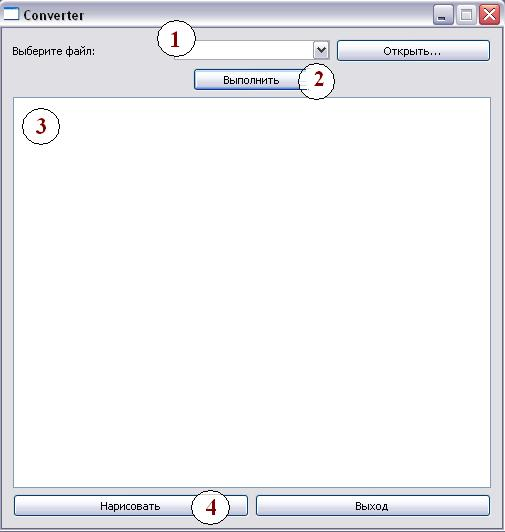
\includegraphics[width=0.7\linewidth]{interface} \\ Рис.1}
\end{figure}

Цифрами 1-4 обозначены области приложения.
\newpage
Приложение в совокупности с подключенной библиотекой обладает \linebreak
следующими возможностями:
\begin{itemize}
\item Область 1. Выбор интересующего файла OSM XML для извлечения  \linebreak
из него нужной
геоинформации (см. Рис.2).

\begin{figure}[h!]
\center{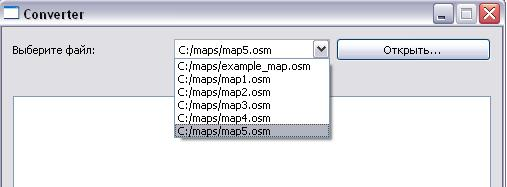
\includegraphics[width=0.7\linewidth]{interface_choose} \\ Рис.2}
\end{figure}

\item Область 2. Кнопка начала извлечения геоданных.

\item Область 3. Просмотр извлеченной геоинформации и занесение  \linebreak
геоданных в базу
данных в формате OpenGIS (см. Рис.3).

\begin{figure}[h!]
\center{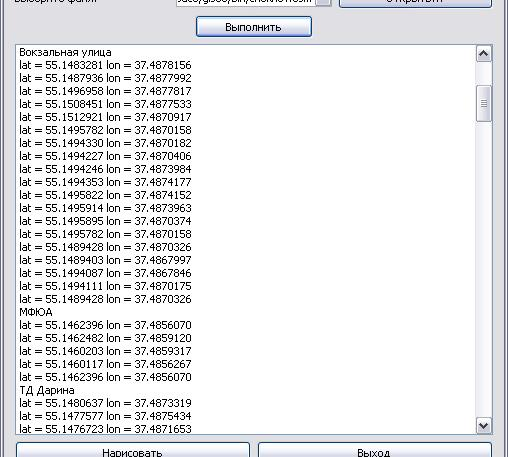
\includegraphics[width=0.7\linewidth]{interface_area} \\ Рис.3}
\end{figure}

\newpage
\item Область 4. Кнопка вызова нового окна приложения, в котором  \linebreak
схематично представляется извлеченная геоинформация (см. Рис.4).

\begin{figure}[h!]
\center{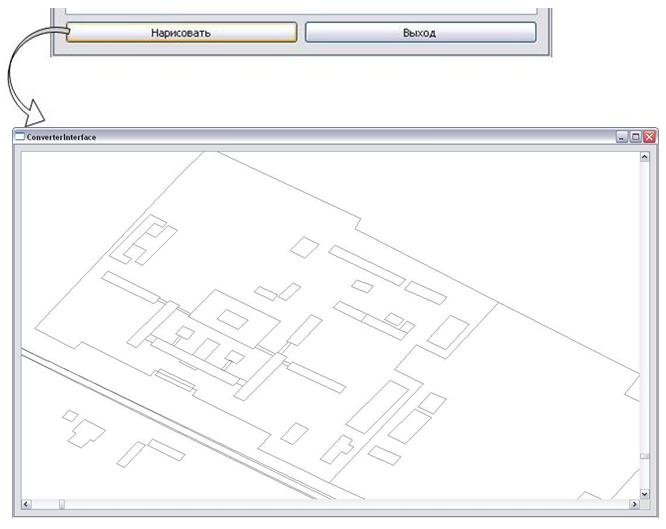
\includegraphics[width=1\linewidth]{interface_on_screen} \\ Рис.4}
\end{figure}

\end{itemize}

Пример работы модуля приведен в Приложении С.

Разработанная библиотека может быть подключена к любому другому \linebreak
приложению, как отдельный независимый переносимый модуль.

%К: практическая часть
%Н: выводы
\newpage
\section{Выводы}
При выполнении учебно-исследовательской работы пройдены основные  \linebreak
этапы разработки специализированного прикладного программного  \linebreak
обеспечения преобразования геоданных из формата OpenStreetMap  \linebreak
в формат OpenGIS:
\begin{itemize}
\item формализация задачи;
\item сбор и обобщение необходимых исходных данных, используемых в \linebreak
программе;
\item составление блок-схемы алгоритма решения задачи;
\item написание и редакция программного кода.
\end{itemize}
В процессе выполнения работы выполнены следующие шаги:
\begin{enumerate}
\item Изучение структуры документа OSM XML и анализ геоданных, \linebreak
хранимых в данном документе.
\item Изучение синтаксиса и возможностей языка XPath. Формирование \linebreak
XPath-запросов для извлечения геоданных об объектах указанного типа.
\item Изучение особенностей СУБД PostgreSQL и её расширения PostGiS.
\item Изучение языка SQL. Формирование SQL-запросов для занесения в \linebreak
базу данных необходимой геоинформации.
\item Разработка модуля на языке C++ с помощью библиотеки Qt.
\end{enumerate}
Разработанный программный модуль :
\begin{itemize}
\item может являться основой для разработки геоинформационных систем \linebreak
различных областей применения;
\item позволяет оптимизировать работу разработчика ГИС путем получения \linebreak
исходных данных в стандартном формате OpenGIS.
\end{itemize}
Исходный код модуля написан на языке Visual C++ и представлен в \linebreak
практической части.

Программа разработана в кросс-платформенной среде разработки - \linebreak
Qt Creator 4.7.4.

Пояснительная записка набрана в LaTeXe при помощи программы WinEdt \linebreak
и оттранслирована в формат '.pdf' при помощи пакета MikTeX.
%К: выводы
%Н: приложение
\newpage
\section{Приложение}
\subsection{Приложение А. Список осей и функций XPath}

\textbf{Оси XPath.}
\begin{itemize}
\item ancestor:: — Возвращает множество предков.
\item ancestor-or-self:: — Возвращает множество предков и текущий элемент.
\item attribute:: — Возвращает множество атрибутов текущего элемента.
\item child:: — Возвращает множество потомков на один уровень ниже.
\item descendant:: — Возвращает полное множество потомков.
\item descendant-or-self:: — Возвращает полное множество потомков и текущий  \linebreak
    элемент.
\item following:: — Возвращает необработанное множество, ниже текущего  \linebreak
элемента.
\item following-sibling:: — Возвращает множество элементов на том же  \linebreak
уровне, следующих за текущим.
\item namespace:: — Возвращает множество имеющее пространство имён  \linebreak
(то есть присутствует атрибут xmlns).
\item parent:: — Возвращает предка на один уровень назад.
\item preceding:: — Возвращает множество обработанных элементов исключая  \linebreak
множество предков.
\item preceding-sibling:: — Возвращает множество элементов на том же уровне,  \linebreak
    предшествующих текущему.
\item self:: — Возвращает текущий элемент.
\end{itemize}

\textbf{Системные функции.}

\begin{itemize}
\item node-set document(object, node-set?) - возвращает документ,  \linebreak
указанный в параметре object.
\item string format-number(number, string, string?) - форматирует  \linebreak
число согласно образцу, указанному во втором параметре, третий  \linebreak
параметр указывает именованный формат числа, который должен быть учтён.
\item string generate-id(node-set?) - возвращает строку, являющуюся  \linebreak
уникальным идентификатором.
\item node-set key(string, object) - возвращает множество с указанным ключом (аналогично функции id для идентификаторов).
\item string unparsed-entity-uri(string) - возвращает непроанализированный URI,  \linebreak
если такового нет, возвращает пустую строку.
\item boolean element-available(string) - проверяет, доступен ли элемент или  \linebreak
    множество, указанное в параметре. Параметр рассматривается как XPath.
\item boolean function-available(string) - проверяет, доступна ли функция,  \linebreak
указанная в параметре. Параметр рассматривается как XPath.
\item object system-property(string) - параметры, возвращающие системные  \linebreak
переменные, могут быть:
- xsl:version — возвращает версию XSLT процессора.

- xsl:vendor — возвращает производителя XSLT процессора.

- xsl:vendor-url — возвращает URL, идентифицирующий производителя.

Если используется неизвестный параметр, функция возвращает пустую строку.

\item boolean lang(string) - возвращает истину, если у текущего тега имеется  \linebreak
атрибут xml:lang, либо родитель тега имеет атрибут xml:lang и в нем  \linebreak
указан совпадающий строке символ.
\end{itemize}

\textbf{Функции с множествами.}

* — обозначает любое имя или набор символов, @* — любой атрибут.

\$name - обращение к переменной, где name — имя переменной  \linebreak
или параметра.

[] — дополнительные условия выборки.

\{\} — если применяется внутри тега другого языка (например HTML),  \linebreak
то XSLT процессор рассматривает содержимое фигурных скобок как XPath.

/ — определяет уровень дерева.
\begin{itemize}
\item node-set node() - возвращает все узлы. Для этой функции часто  \linebreak
используют заменитель '*', но в отличие от звездочки — node()  \linebreak
возвращает и текстовые узлы.
\item string text() - возвращает набор текстовых узлов
\item node-set current() - возвращает множество из одного элемента,  \linebreak
который является текущим. Если мы делаем обработку множества с  \linebreak
условиями, то единственным способом дотянуться из этого условия  \linebreak
до текущего элемента будет данная функция.
\item number position() - возвращает позицию элемента в множестве. \linebreak
 Корректно работает только в цикле <xsl:for-each/>
\item number last() - возвращает номер последнего элемента в  \linebreak
множестве. Корректно работает только в цикле <xsl:for-each/>
\item number count(node-set) - возвращает количество элементов в node-set.
\item string name(node-set?) - возвращает полное имя первого тега  \linebreak
в множестве.
\item string namespace-uri(node-set?) - возвращает ссылку на url  \linebreak
определяющий пространство имён.
\item string local-name(node-set?) - возвращает имя первого тега  \linebreak
в множестве, без пространства имён.
\item node-set id(object) - находит элемент с уникальным идентификатором
\end{itemize}

\textbf{Строковые функции.}

\begin{itemize}
\item string string(object?) - возвращает текстовое содержимое элемента. \linebreak
 По сути возвращает объединенное множество текстовых элементов на  \linebreak
 один уровень ниже.
\item string concat(string, string, string*) - объединяет две или более строк
\item number string-length(string?) - возвращает длину строки.
\item boolean contains(string, string) - возвращает истину, если первая  \linebreak
строка содержит вторую, иначе возвращает ложь.
\item string substring(string, number, number?) - возвращает строку  \linebreak
вырезанную из строки начиная с указанного номера, и если указан  \linebreak
второй номер — количество символов.
\item string substring-before(string, string) - если найдена вторая строка  \linebreak
в первой, возвращает строку до первого вхождения второй строки.
\item string substring-after(string, string) - если найдена вторая строка  \linebreak
в первой, возвращает строку после первого вхождения второй строки.
\item boolean starts-with(string, string) - возвращает истину, если  \linebreak
вторая строка входит в начало первой, иначе возвращает ложь.
\item boolean ends-with(string, string) - возвращает истину, если  \linebreak
вторая строка входит в конец первой, иначе возвращает ложь.
\item string normalize-space(string?) - убирает лишние и повторные  \linebreak
пробелы, а также управляющие символы, заменяя их пробелами.
\item string translate(string, string, string) - заменяет символы первой  \linebreak
строки, которые встречаются во второй строке, на соответствующие  \linebreak
позиции символам из второй строки символы из третьей строки.  \linebreak
\end{itemize}

\textbf{Логические функции}

\begin{itemize}
\item or — логическое «или»
\item and — логическое «и»
\item = — логическое «равно»
\item < (\&lt;) — логическое "меньше"
\item > (\&gt;) — логическое "больше"
\item <= (\&lt;=) — логическое "меньше либо равно"
\item >= (\&gt;=) — логическое "больше либо равно"
\end{itemize}

\textbf{Числовые функции}

\begin{itemize}
\item + — сложение
\item - — вычитание
\item * — умножение
\item div — обычное деление (не деление нацело!)
\item mod — остаток от деления
\end{itemize}
\newpage
\subsection{Приложение B. Программный код модуля.}

\newpage
\subsection{Приложение С. Пример работы модуля.}
Для демонстрации работы модуля рассмотрим OSM-файл, в котором \linebreak
содержится информация о территории МИФИ.

Выбираем файл 'map\_mephi.osm'.

\begin{figure}[h!]
\center{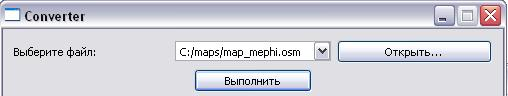
\includegraphics[width=0.7\linewidth]{map_mephi_choose}}
\end{figure}

Нажатием кнопки 'Выполнить' происходит разбор OSM-файла.

\begin{figure}[h!]
\center{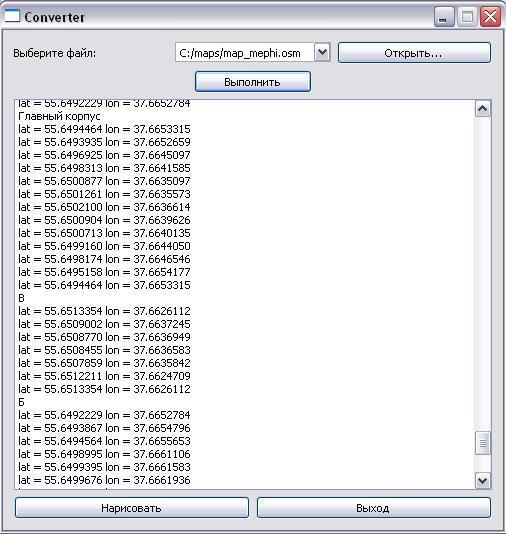
\includegraphics[width=0.7\linewidth]{map_mephi_area}}
\end{figure}

Совместно с этим действием происходит занесение геоданных в базу \linebreak
данных. С помощью открытого графического инструмента \linebreak
администрирования PostgreSQL для Windows pgAdmin можно посмотреть, \linebreak
какие данные занесены в таблицы tags и objects.

\newpage
Содержимое таблицы objects:
\begin{figure}[h!]
\center{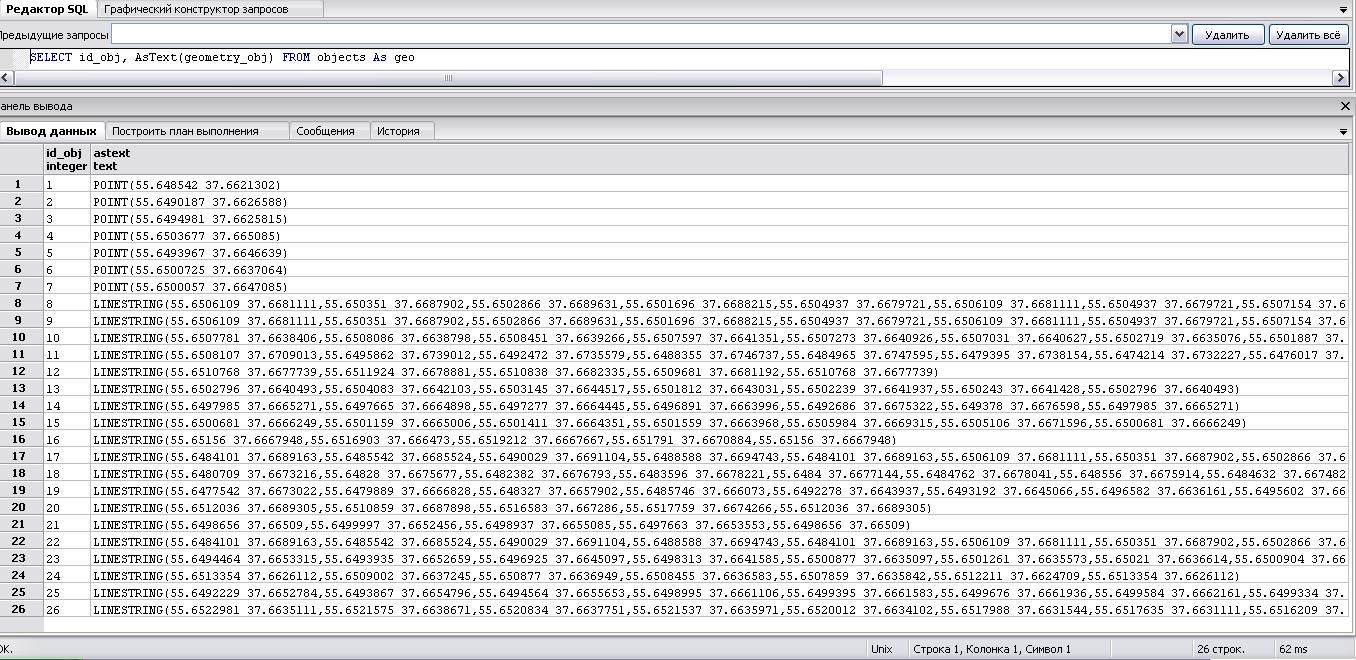
\includegraphics[width=1.1\linewidth]{map_mephi_bd_objects}}
\end{figure}

Содержимое таблицы tags:
\begin{figure}[h!]
\center{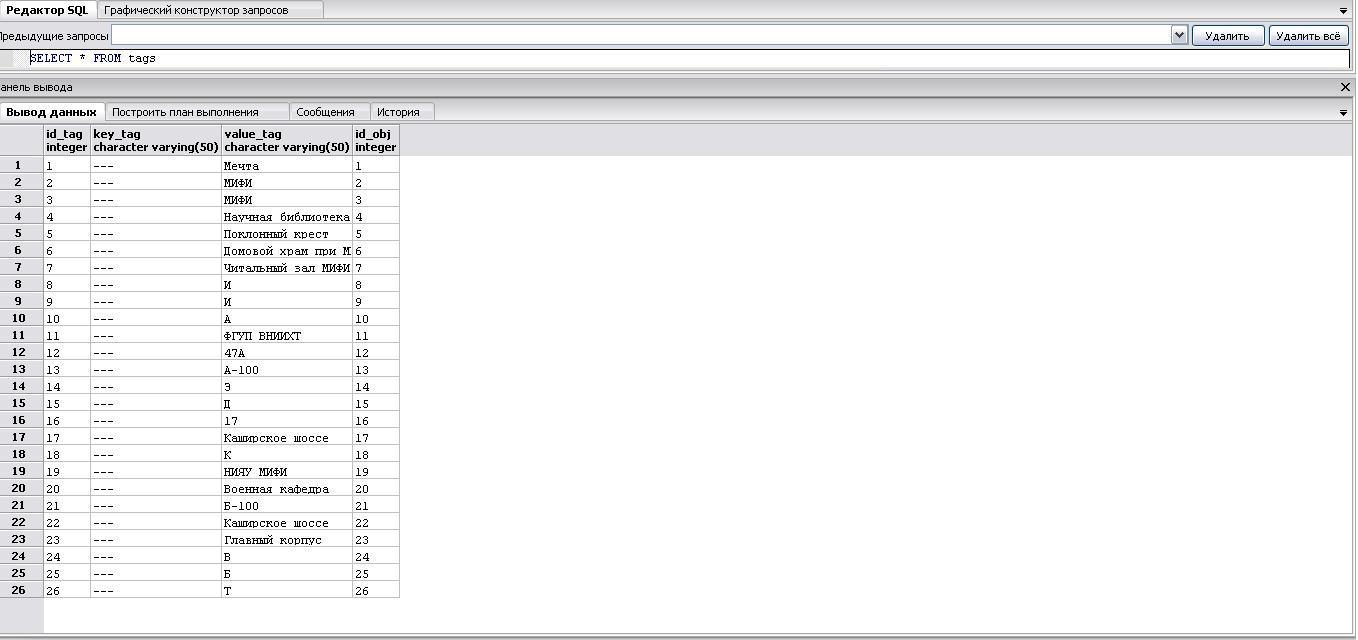
\includegraphics[width=1\linewidth]{map_mephi_bd_tags}}
\end{figure}
\newpage
Рассмотрим объект 'Главный корпус'. Он представляется в \linebreak
OSM-документе следующим образом:
\vskip--10pt
Главный корпус

lat = 55.6494464 lon = 37.6653315

lat = 55.6493935 lon = 37.6652659

lat = 55.6496925 lon = 37.6645097

lat = 55.6498313 lon = 37.6641585

lat = 55.6500877 lon = 37.6635097

lat = 55.6501261 lon = 37.6635573

lat = 55.6502100 lon = 37.6636614

lat = 55.6500904 lon = 37.6639626

lat = 55.6500713 lon = 37.6640135

lat = 55.6499160 lon = 37.6644050

lat = 55.6498174 lon = 37.6646546

lat = 55.6495158 lon = 37.6654177

lat = 55.6494464 lon = 37.6653315
\vskip--10pt

В базу данных этот объект занесен в таблицу tags с \linebreak
идентификатором '23' c атрибутом 'name = Главный корпус' и \linebreak
ссылкой на запись таблицы objects с идентификатором '23'. \linebreak
Под этим идентификатором в таблице objects хранятся координаты \linebreak
объекта 'Главный корпус', а именно:
\vskip--10pt
'LINESTRING(55.6494464 37.6653315,55.6493935 37.6652659,\linebreak
55.6496925 37.6645097,55.6498313 37.6641585,55.6500877 37.6635097,\linebreak
55.6501261 37.6635573,55.65021 37.6636614,...)'

В базе данных объект хранится в виде, соответствующем спецификации OpenGIS.
\vskip--10pt
\newpage
Графическое представление извлеченных данных.
\begin{figure}[h!]
\center{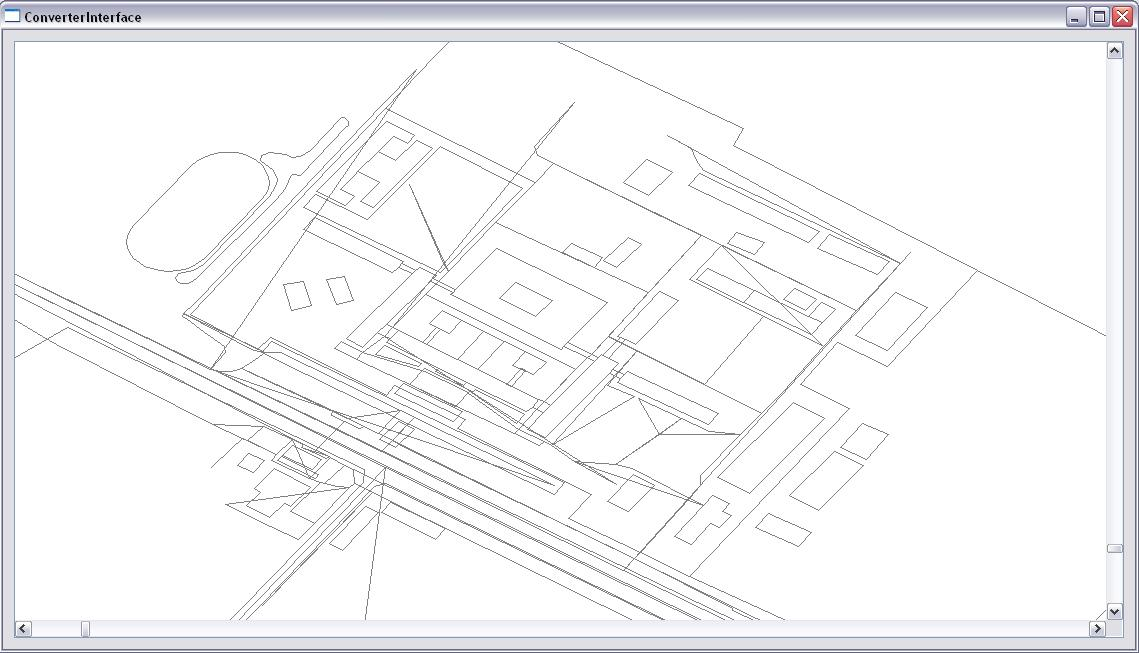
\includegraphics[width=1\linewidth]{map_mephi}}
\end{figure}
%К: приложение
\end{document} 